% Tiểu luận rút gọn. Biên dịch bằng XeLaTeX (Tectonic): tectonic -X compile main.tex
\documentclass[a4paper,12pt,oneside]{report}
\usepackage[fontsize=13pt]{scrextend}

% ── Công thức: Times (mathptmx); chữ: Times New Roman ──────────────────
\usepackage{amsmath,amssymb}
\usepackage{mathptmx}
\usepackage{dsfont}
\usepackage[no-math]{fontspec}
\setmainfont{Times New Roman}
\setmonofont{Liberation Mono}[Scale=0.85]
\usepackage{polyglossia}
\setdefaultlanguage{vietnamese}

% ── Trang, lề, giãn dòng ──────────────────────────────────────────────
\usepackage[a4paper,left=3cm,right=2cm,top=2.5cm,bottom=2.5cm,footskip=1.2cm]{geometry}
\usepackage{setspace}
\onehalfspacing
\usepackage{indentfirst}
\setlength{\parindent}{1.27cm}
\setlength{\parskip}{2pt}
\setlength{\emergencystretch}{3em}

% ── Tiêu đề ───────────────────────────────────────────────────────────
\setcounter{secnumdepth}{1}
\usepackage{titlesec}
\titleformat{\chapter}[block]{\fontsize{14}{18}\selectfont\bfseries\centering}
  {\MakeUppercase{\chaptertitlename}~\thechapter.}{0.4em}{\MakeUppercase}
\titlespacing{\chapter}{0pt}{0pt}{12pt}
\titleformat{\section}[block]{\fontsize{13}{16}\selectfont\bfseries\raggedright}{\thesection.}{0.4em}{}
\titlespacing{\section}{0pt}{8pt}{3pt}
\titleformat{\subsection}[block]{\fontsize{13}{16}\selectfont\bfseries\raggedright}{}{0pt}{}
\titlespacing{\subsection}{1.27cm}{6pt}{2pt}

% ── Chân trang: tên chương (trái, nghiêng) | số trang (phải) ──────────
\usepackage{fancyhdr}
\pagestyle{fancy}
\fancyhf{}
\fancyfoot[L]{\small\itshape\nouppercase{\leftmark}}
\fancyfoot[R]{\thepage}
\renewcommand{\headrulewidth}{0pt}
\renewcommand{\chaptermark}[1]{\markboth{Chương~\thechapter. #1}{}}
\renewcommand{\sectionmark}[1]{}
\fancypagestyle{plain}{\fancyhf{}\fancyfoot[L]{\small\itshape\nouppercase{\leftmark}}\fancyfoot[R]{\thepage}}
\newcommand{\unnumbered}[1]{\chapter*{#1}\addcontentsline{toc}{chapter}{#1}\markboth{#1}{}}

% ── Danh sách: ● cấp 1, – cấp 2 ───────────────────────────────────────
\usepackage{enumitem}
\setlist{itemsep=1pt,parsep=0pt,topsep=2pt}
\setlist[itemize,1]{label={\small\textbullet},leftmargin=1.27cm}
\setlist[itemize,2]{label={\textendash},leftmargin=0.8cm}
\setlist[enumerate,1]{leftmargin=1.27cm}

% ── Bảng, hình, chú thích ─────────────────────────────────────────────
\usepackage{array,tabularx,graphicx,float,tikz}
\newcolumntype{R}{>{\raggedleft\arraybackslash}X}
\newcolumntype{L}{>{\raggedright\arraybackslash}X}
\newenvironment{tbl}{\par\small\setstretch{1.1}\renewcommand{\arraystretch}{1.2}\centering}{\par}
\usepackage[labelsep=period,font=small,skip=4pt]{caption}
\captionsetup[figure]{font={small,it}}
\renewcommand{\thefigure}{\thechapter.\arabic{figure}}
\renewcommand{\thetable}{\thechapter.\arabic{table}}
\renewcommand{\theequation}{\thechapter.\arabic{equation}}

% ── Mục lục ───────────────────────────────────────────────────────────
\usepackage{tocloft}
\setcounter{tocdepth}{1}
\renewcommand{\cfttoctitlefont}{\hfill\fontsize{14}{18}\selectfont\bfseries\MakeUppercase}
\renewcommand{\cftaftertoctitle}{\hfill}
\renewcommand{\cftchapdotsep}{\cftdotsep}
\renewcommand{\cftchapfont}{\bfseries}
\renewcommand{\cftchappresnum}{Chương }
\renewcommand{\cftchapaftersnum}{.}
\setlength{\cftchapnumwidth}{5.6em}
\renewcommand{\cftsecaftersnum}{.}
\setlength{\cftbeforechapskip}{3pt}
\renewcommand{\cftmarktoc}{\markboth{Mục lục}{}}

\usepackage[hidelinks]{hyperref}
\hypersetup{pdftitle={Ứng dụng kiến trúc Delta Lake và Apache Spark trong xử lý dữ liệu lớn và xây dựng hệ thống gợi ý sản phẩm},
  pdfauthor={Nguyễn Hoàng Vũ Thân},colorlinks=true,linkcolor=black,citecolor=black,urlcolor=blue!50!black}

\begin{document}

% ════════════════════════════ TRANG BÌA ════════════════════════════════
\begin{titlepage}
\begin{tikzpicture}[remember picture,overlay]
  \draw[line width=1.6pt] ([xshift=2.4cm,yshift=-1.9cm]current page.north west) rectangle ([xshift=-1.4cm,yshift=1.9cm]current page.south east);
  \draw[line width=0.5pt] ([xshift=2.55cm,yshift=-2.05cm]current page.north west) rectangle ([xshift=-1.55cm,yshift=2.05cm]current page.south east);
\end{tikzpicture}
\centering\singlespacing
{\fontsize{16}{22}\selectfont\bfseries BỘ GIÁO DỤC VÀ ĐÀO TẠO\\[2pt] TRƯỜNG ĐẠI HỌC QUY NHƠN\par}
\vfill

\includegraphics[width=5cm]{figures/logo_dhqn.png}\par
\vfill
{\fontsize{19}{28}\selectfont\bfseries ỨNG DỤNG KIẾN TRÚC DELTA LAKE VÀ APACHE SPARK TRONG XỬ LÝ DỮ LIỆU LỚN VÀ XÂY DỰNG HỆ THỐNG GỢI Ý SẢN PHẨM\par}
\vspace{14pt}
{\fontsize{14}{20}\selectfont\itshape Building a Product Recommendation System Using Delta Lake and Apache Spark\par}
\vfill
{\fontsize{14}{22}\selectfont
\begin{tabular}{@{}ll@{}}
\textbf{Môn học:} & Khai phá dữ liệu lớn (Big Data Mining) \\
\textbf{Giảng viên:} & TS. Trần Thiên Thành \\
\textbf{Học viên:} & Nguyễn Hoàng Vũ Thân \\
\textbf{Mã học viên:} & 8282548015 \\
\textbf{Lớp:} & KHDL28B (Thạc sĩ) \\
\end{tabular}\par}
\vfill
{\itshape Tháng 10 năm 2026\par}
\end{titlepage}

\pagenumbering{roman}
\tableofcontents
\clearpage
\pagenumbering{arabic}

% ════════════════════════════ MỞ ĐẦU ═══════════════════════════════════
\unnumbered{Mở đầu}

\subsection*{1. Lý do chọn đề tài}
Các sàn thương mại điện tử ghi lại hàng trăm triệu lượt xem, thêm giỏ hàng và mua mỗi năm. Khai thác được nguồn dữ liệu này đòi hỏi hai năng lực đi cùng nhau: một hạ tầng lưu trữ và xử lý có kiểm soát (nạp lại không trùng lặp, truy vết được phiên bản dữ liệu đã dùng) và một mô hình gợi ý được đánh giá trung thực. Kiến trúc lakehouse với Delta Lake trên object storage, kết hợp Apache Spark, là cách tiếp cận phổ biến cho yêu cầu thứ nhất; lọc cộng tác bằng phân rã ma trận là phương pháp kinh điển cho yêu cầu thứ hai. Đề tài kết hợp hai hướng này trên một bộ dữ liệu bán lẻ thật, trong điều kiện tài nguyên hạn chế của một máy tính cá nhân.

\subsection*{2. Mục tiêu}
\begin{itemize}
  \item Xây dựng pipeline xử lý batch theo kiến trúc Medallion (Bronze, Silver, Gold) trên Delta Lake và MinIO bằng Spark, có kiểm chứng tính toàn vẹn và khả năng tái lập.
  \item Tổ chức kho dữ liệu theo mô hình Star Schema phục vụ phân tích bằng Spark SQL, và một data mart riêng cho học máy.
  \item Huấn luyện mô hình Implicit ALS trên GPU, so sánh với mô hình phổ biến (Popularity) theo giao thức chia thời gian chặt chẽ.
  \item Đo thời gian và tài nguyên của toàn bộ quy trình.
\end{itemize}

\subsection*{3. Đối tượng và phạm vi}
Đối tượng là miền Retail của bộ dữ liệu T-ECD Small~\cite{tecd}: 267.043.972 sự kiện của 140.062 người dùng trên 257.327 sản phẩm trong 227 ngày. Đề tài chỉ xử lý batch trên một máy, không xây dựng dịch vụ gợi ý trực tuyến.

\subsection*{4. Phương pháp thực hiện}
Đề tài theo hướng thực nghiệm. Toàn bộ mã nguồn, kết quả và lập luận nằm trong một notebook Jupyter chạy theo từng giai đoạn có checkpoint. Mọi số liệu trong bài lấy từ một lượt chạy đầy đủ trên toàn bộ dữ liệu Retail.

\subsection*{5. Bố cục}
Ngoài phần mở đầu và kết luận, tiểu luận gồm ba chương: Chương 1 trình bày cơ sở lý thuyết; Chương 2 mô tả dữ liệu, kiến trúc và các tầng xử lý dữ liệu; Chương 3 trình bày việc xây dựng, đánh giá mô hình gợi ý và hiệu năng hệ thống.

% ════════════════════════ CHƯƠNG 1 ═════════════════════════════════════
\chapter{Cơ sở lý thuyết}

\section{Apache Spark, Delta Lake và MinIO}
Apache Spark là nền tảng xử lý dữ liệu phân tán, mô tả phép biến đổi bằng DataFrame và Spark SQL rồi chỉ thực thi khi có hành động như ghi bảng hay đếm dòng~\cite{spark,sparksql}. Delta Lake bổ sung nhật ký giao dịch cho các file Parquet, nhờ đó có giao dịch ACID, kiểm soát schema và đọc lại dữ liệu theo phiên bản (time travel)~\cite{delta,deltadocs}. MinIO là object storage tương thích S3, được Spark truy cập qua Hadoop S3A~\cite{s3a}. Trong hệ thống, ba thành phần chia vai rõ ràng: MinIO lưu trữ, Delta quản lý bảng, Spark xử lý.

\section{Kiến trúc Medallion và mô hình Star Schema}
Kiến trúc Medallion~\cite{medallion} tổ chức dữ liệu theo mức độ tinh luyện: Bronze giữ dữ liệu gốc kèm thông tin nguồn; Silver chứa dữ liệu đã làm sạch, chuẩn hóa; Gold chứa dữ liệu sẵn sàng cho phân tích và mô hình. Ở tầng Gold, đề tài dùng mô hình Star Schema của Kimball~\cite{kimball}: một bảng fact ở mức chi tiết nhất (mỗi dòng là một sự kiện) nối với các bảng dimension mô tả. Star Schema được chọn thay cho Snowflake vì các dimension nhỏ (lớn nhất là bảng sản phẩm với 259.377 dòng), thuộc tính sản phẩm chỉ có hai cấp ngành hàng, và mọi truy vấn phân tích chỉ cần một bước nối từ fact.

\section{Lọc cộng tác từ phản hồi ngầm và Implicit ALS}
Dữ liệu bán lẻ chỉ có phản hồi ngầm (xem, nhấp, thêm giỏ, mua), không có điểm đánh giá. Phân rã ma trận~\cite{koren} biểu diễn mỗi user $u$ và item $i$ bằng vector nhân tố $x_u, y_i \in \mathbb{R}^k$. Hu và cộng sự~\cite{hu} tách sở thích nhị phân $p_{ui}=\mathds{1}[r_{ui}>0]$ khỏi độ tin cậy $c_{ui}=1+\alpha r_{ui}$, trong đó $r_{ui}$ là cường độ tương tác, và cực tiểu hóa
\begin{equation}
\min_{X,Y}\sum_{u,i}c_{ui}\left(p_{ui}-x_u^{T}y_i\right)^2+\lambda\Big(\sum_u\|x_u\|^2+\sum_i\|y_i\|^2\Big).
\end{equation}
Khi cố định $Y$, bài toán tách thành các hệ tuyến tính $k\times k$ độc lập cho từng user:
\begin{equation}
A_u x_u=b_u,\qquad A_u=G+\sum_{i\in I_u}\alpha r_{ui}\,y_iy_i^{T}+\lambda I,\qquad b_u=\sum_{i\in I_u}(1+\alpha r_{ui})\,y_i,
\end{equation}
với $G=Y^{T}Y$ tính một lần cho mọi user và $I_u$ là tập item user đã tương tác. Vì vậy không cần dựng ma trận đặc user~$\times$~item. Cập nhật item làm tương tự với vai trò của $X$ và $Y$ đổi chỗ.

Thay vì giải trực tiếp, Takács và cộng sự~\cite{takacs} dùng phương pháp gradient liên hợp (CG), chỉ cần tích $A_uq$ mà không phải dựng $A_u$. Backend CUDA của đề tài chạy tối đa $s=5$ bước CG cho mỗi lần cập nhật, khởi động từ nghiệm của vòng trước. Gọi $N$ là số cặp user–item khác 0, $m$ và $n$ là số user và item, chi phí một lượt cập nhật user là
\begin{equation}
O\!\left(nk^2\right)+O\!\left((s+1)(mk^2+Nk)\right),
\end{equation}
so với $O(Nk^2+mk^3)$ khi giải trực tiếp. Hệ quả quan trọng cho thiết kế: thời gian huấn luyện tỉ lệ với số cặp khác 0, không phải với số dòng sự kiện.

\section{Đánh giá hệ gợi ý Top-N}
Với tập item user thực sự mua $R_u$ và danh sách gợi ý $L_u$ gồm tối đa $K=10$ item, hai độ đo được dùng là~\cite{rankingmetrics,ndcg}
\begin{equation}
\mathrm{Recall@}K(u)=\frac{|L_u\cap R_u|}{|R_u|},\qquad
\mathrm{NDCG@}K(u)=\frac{1}{\mathrm{IDCG@}K(u)}\sum_{j=1}^{|L_u|}\frac{\mathds{1}[L_{u,j}\in R_u]}{\log_2(j+1)},
\end{equation}
trong đó IDCG là giá trị DCG lớn nhất có thể đạt. Điểm được lấy trung bình theo user và xếp hạng trên toàn bộ tập ứng viên, vì đánh giá trên tập ứng viên lấy mẫu có thể đảo thứ hạng các mô hình~\cite{krichene}. Các nghiên cứu~\cite{cremonesi,dacrema} cho thấy mô hình đơn giản như Popularity (gợi ý các sản phẩm được mua nhiều nhất) thường rất khó vượt, nên mọi mô hình phải được so sánh với nó trên cùng tập user, nhãn và ứng viên. Với hàng tiêu dùng, hành vi mua lặp lại~\cite{repeat} cũng là đặc điểm cần tính đến khi thiết kế đánh giá.

% ════════════════════════ CHƯƠNG 2 ═════════════════════════════════════
\chapter{Dữ liệu và kiến trúc hệ thống}

\section{Bộ dữ liệu T-ECD Retail}
T-ECD là bộ dữ liệu thương mại điện tử đã được ẩn danh và gây nhiễu có kiểm soát~\cite{tecd}. Miền Retail gồm 227 file sự kiện theo ngày và một file danh mục sản phẩm (Bảng~\ref{tab:data}). Thời gian chỉ là tọa độ tương đối nên đề tài không suy diễn ngày lịch thực. Dữ liệu không có mã đơn hàng hay số lượng, vì vậy sự kiện \texttt{order} được hiểu là một lần mua, không dùng để tính doanh thu. Có 8.521 sản phẩm xuất hiện trong sự kiện nhưng thiếu trong danh mục, và 99\% giá trong danh mục là số âm do đã biến đổi.

\begin{table}[!htbp]
\caption{Thông tin chính của dữ liệu T-ECD Small, miền Retail}\label{tab:data}
\begin{tbl}
\begin{tabularx}{\linewidth}{|l|L|}
\hline
\textbf{Thuộc tính} & \textbf{Giá trị} \\ \hline
Quy mô & 267.043.972 sự kiện; 140.062 user; 257.327 item; 227 ngày (1082–1308); 2,13 GB Parquet \\ \hline
Hành vi & view 94,9\% · order 2,78\% · added\_to\_cart 1,44\% · click 0,86\% \\ \hline
Ngữ cảnh & OS: android 90,8\%, ios 8,2\%; subdomain: catalog 86,6\%, search 8,1\% \\ \hline
Danh mục & 250.856 sản phẩm: brand, category, subcategory, giá, embedding 300 chiều \\ \hline
\end{tabularx}
\end{tbl}
\end{table}

\section{Kiến trúc tổng thể}
Hình~\ref{fig:arch} mô tả luồng dữ liệu. Spark nạp file nguồn vào Bronze, làm sạch sang Silver, rồi tạo hai nhóm bảng Gold: kho dữ liệu Star Schema cho phân tích bằng Spark SQL, và ML Data Mart cho huấn luyện. Mô hình ALS và việc sinh danh sách Top-10 chạy trên GPU bằng CuPy, ngoài JVM của Spark. Tất cả bảng đều là bảng Delta trên MinIO.

\begin{figure}[!htbp]
\centering
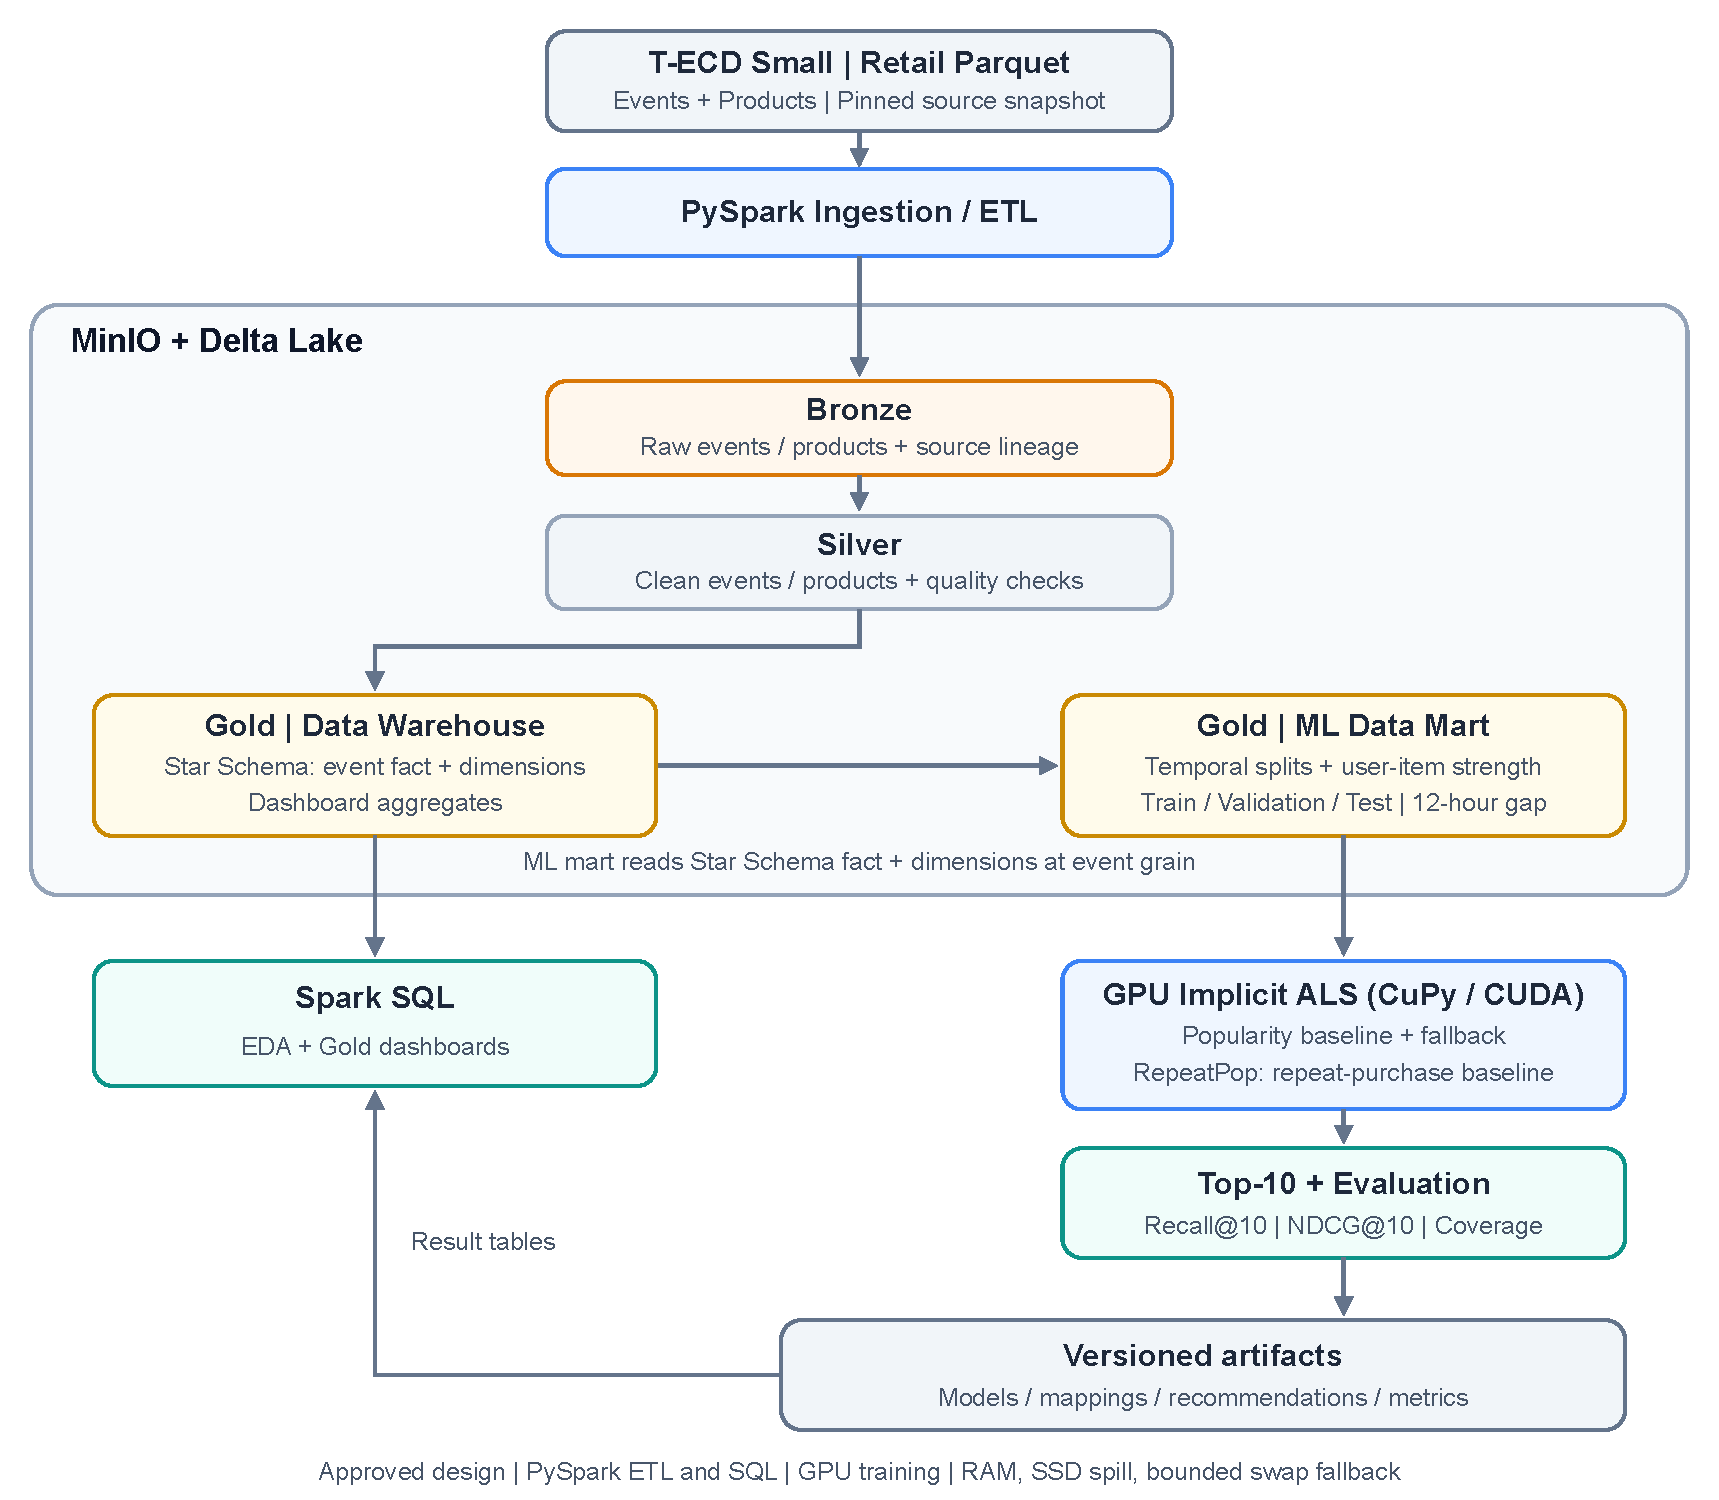
\includegraphics[width=0.78\linewidth]{figures/architecture.pdf}
\caption{Kiến trúc hệ thống: Medallion trên Delta Lake/MinIO, Spark ETL và ALS trên GPU}\label{fig:arch}
\end{figure}

Hệ thống chạy trên một máy tính xách tay có GPU NVIDIA RTX 4050 (6 GiB VRAM), 16 luồng CPU và 16 GB RAM, với PySpark 4.2, Delta Lake 4.4.1~\cite{deltacompat} và CuPy 14.2. Toàn bộ tiến trình bị giới hạn ở 7 GiB RAM và 4 GiB swap; Spark chạy ở chế độ \texttt{local[2]} với heap 3 GiB. Quy trình chia thành 13 giai đoạn, mỗi giai đoạn lưu checkpoint, nên khi bị gián đoạn chỉ cần chạy lại cùng lệnh để tiếp tục.

\section{Tầng Bronze và Silver}
Bronze nạp 227 batch theo ngày, mỗi ngày là một lần ghi Delta có điều kiện thay thế đúng phân vùng ngày đó; mỗi sự kiện được gán khóa kỹ thuật cùng tên file, ngày nguồn và mã batch để truy vết. Quá trình nạp mất 22,8 phút. Năm kiểm tra Delta đều đạt: nạp lại một ngày không nhân đôi dữ liệu; đọc lại phiên bản cũ cho đúng số dòng và schema; khóa bản ghi ổn định khi nạp lại; lịch sử thay đổi ghi đủ các lần commit; ghi sai kiểu dữ liệu bị từ chối. Đây là các tính chất mà phần còn lại của hệ thống dựa vào.

Silver chuẩn hóa kiểu dữ liệu, thay giá trị rỗng của OS và subdomain bằng \texttt{unknown}, và đưa dòng lỗi vào bảng quarantine kèm lý do. Kết quả: toàn bộ 267.043.972 sự kiện hợp lệ, quarantine bằng 0; danh mục giữ một dòng cho mỗi sản phẩm, gắn cờ cho giá trị thiếu hoặc giá âm.

\section{Kho dữ liệu Star Schema và phân tích}
Bảng fact \texttt{fact\_interactions} có mỗi dòng là một sự kiện, nối với năm dimension: user, sản phẩm, ngày, hành vi và ngữ cảnh (OS, subdomain). Mỗi sản phẩm thiếu danh mục có một dòng Unknown riêng trong dimension sản phẩm, nhờ đó phép nối không làm mất sự kiện nào. Các kiểm tra xác nhận khóa của mọi dimension là duy nhất và số dòng fact đúng bằng số dòng Silver. Trên kho này, 10 bảng tổng hợp bằng Spark SQL phục vụ phân tích theo ngày, hành vi, ngành hàng, brand và ngữ cảnh.

Phân tích cho thấy ba đặc điểm ảnh hưởng trực tiếp tới mô hình. Thứ nhất, tín hiệu mua rất thưa: khoảng 34 lượt xem cho mỗi lượt mua. Thứ hai, nhu cầu tập trung mạnh: ngành thực phẩm chiếm 80,7\% sự kiện; 1\% sản phẩm phổ biến nhất chiếm 27,4\% sự kiện, trong khi một nửa số sản phẩm ít phổ biến nhất chỉ chiếm 1,3\% (Hình~\ref{fig:tail}). Thứ ba, mức hoạt động của user lệch nặng: 3\% user nhiều sự kiện nhất tạo ra 56,4\% tổng sự kiện. Ma trận user–item có độ thưa 99,83\%.

\begin{figure}[!htbp]
\centering
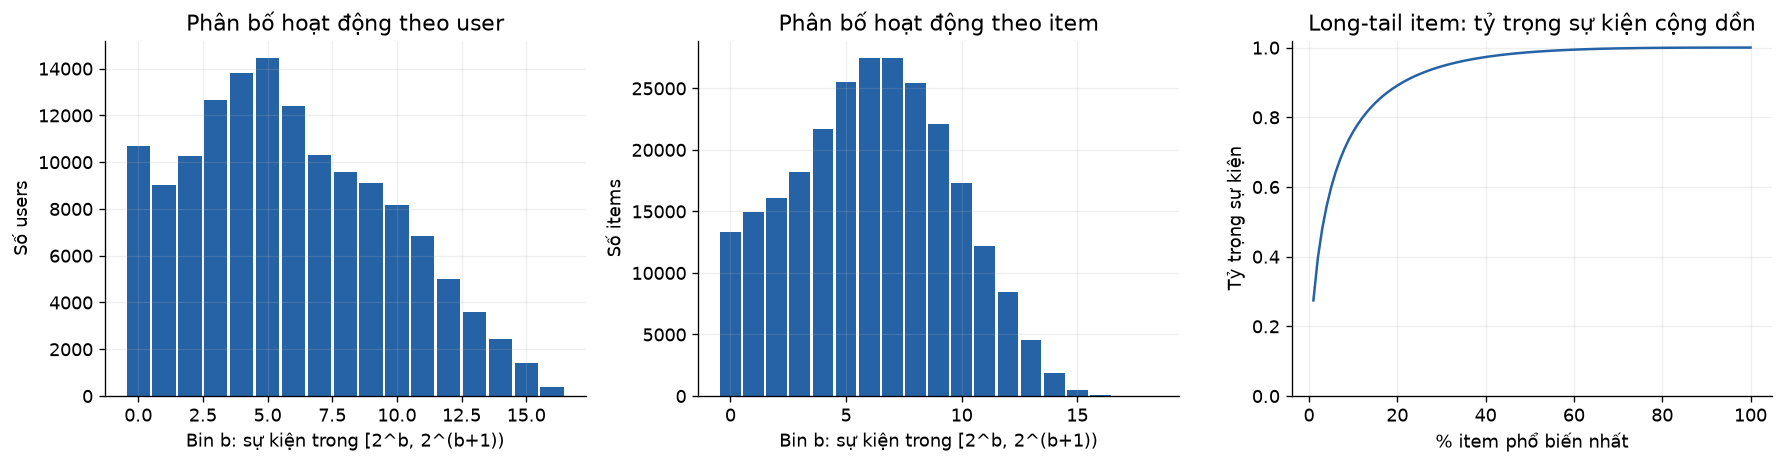
\includegraphics[width=\linewidth]{figures/output_04.png}
\caption{Phân bố hoạt động theo user, theo item và đường cong long-tail}\label{fig:tail}
\end{figure}

\section{Gold ML Data Mart}
Data mart đọc trực tiếp bảng fact ở mức sự kiện và lọc theo mốc thời gian \emph{trước} khi tổng hợp, để không có thông tin nào từ giai đoạn đánh giá lọt vào dữ liệu huấn luyện. Mỗi cặp user–item được tổng hợp thành số sự kiện của từng hành vi; cường độ tương tác $r_{ui}$ là tổng có trọng số của các số đếm này. Hai bộ trọng số được thử: đồng đều (1, 1, 1, 1) và ưu tiên mua (view 1, click 2, thêm giỏ 3, mua 5).

Vì thời gian huấn luyện tỉ lệ với số cặp khác 0 (mục 1.3), data mart bỏ những cặp chỉ có đúng một lượt xem; cặp có nhấp, thêm giỏ hoặc mua luôn được giữ, nên nhãn mua và Popularity không đổi. Trên dữ liệu huấn luyện, số cặp giảm từ 49,8 triệu xuống 20,8 triệu (còn 41,8\%), trong khi vẫn giữ 95,5\% user và 90,8\% item. User mất hết cặp sau bước này được coi như user mới và nhận gợi ý Popularity.

% ════════════════════════ CHƯƠNG 3 ═════════════════════════════════════
\chapter{Xây dựng và đánh giá mô hình gợi ý}

\section{Thiết kế thực nghiệm}
Dữ liệu được chia theo thời gian: 14 ngày cuối là tập kiểm tra (test), 14 ngày trước đó là tập kiểm định (validation). Lịch sử dùng để huấn luyện kết thúc 12 giờ trước ngày đầu của tập tương ứng (Bảng~\ref{tab:split}). Nhãn là các cặp user–item có sự kiện mua trong cửa sổ đánh giá.

\begin{table}[!htbp]
\caption{Giao thức chia dữ liệu theo thời gian}\label{tab:split}
\begin{tbl}
\begin{tabularx}{\linewidth}{|l|l|L|}
\hline
\textbf{Tập} & \textbf{Ngày} & \textbf{Lịch sử huấn luyện tương ứng} \\ \hline
Validation & 1281–1294 & 215.925.462 sự kiện (80,9\%), kết thúc 12 giờ trước ngày 1281 \\ \hline
Test & 1295–1308 & 239.831.885 sự kiện, kết thúc 12 giờ trước ngày 1295 \\ \hline
\end{tabularx}
\end{tbl}
\end{table}

Đánh giá dùng hai quy tắc ứng viên. Quy tắc chính cho phép gợi ý lại sản phẩm user đã tương tác, phù hợp với hàng tiêu dùng mua lặp lại. Quy tắc phụ loại sản phẩm user đã tương tác khỏi cả danh sách ứng viên lẫn nhãn, để đo khả năng gợi ý sản phẩm mới. Ứng viên là các sản phẩm có trong lịch sử sau rút gọn (221.967 ở validation, 227.442 ở test); nhãn ngoài tập này vẫn được tính trong mẫu số. Popularity xếp hạng sản phẩm theo số lượt mua trong cùng lịch sử. Để tránh dùng tập test cho việc lựa chọn, giao thức được khóa trước khi huấn luyện, và cấu hình ALS được chọn trên validation rồi khóa trước khi chạy test.

\section{Lựa chọn cấu hình ALS}
Lưới khảo sát gồm 16 cấu hình: hai bộ trọng số $\times$ rank $k\in\{32,64\}$ $\times$ $\lambda\in\{0{,}05;\,0{,}1\}$ $\times$ $\alpha\in\{10,40\}$, mỗi cấu hình chạy 10 vòng với seed 42. Hình~\ref{fig:e2} cho thấy cấu hình tốt nhất là trọng số đồng đều, $k=32$, $\lambda=0{,}1$, $\alpha=10$ với NDCG@10 = 0,1488, nhưng vẫn thấp hơn Popularity trên cùng validation (0,1741).

\begin{figure}[!htbp]
\centering
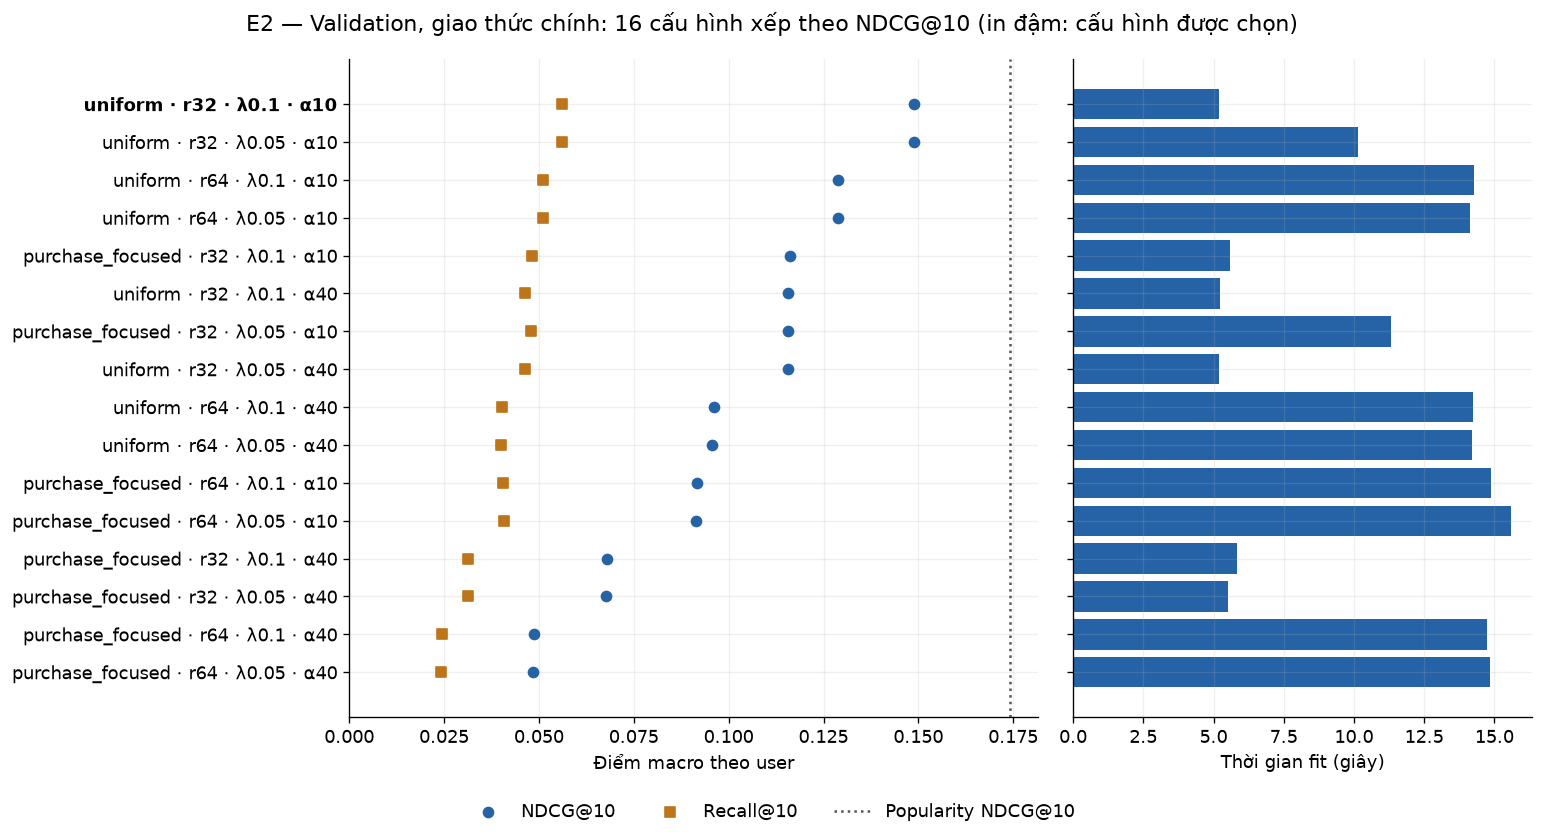
\includegraphics[width=\linewidth]{figures/output_06.png}
\caption{Kết quả 16 cấu hình ALS trên validation, xếp theo NDCG@10, kèm thời gian huấn luyện}\label{fig:e2}
\end{figure}

Ảnh hưởng của từng tham số rất nhất quán. Khi các yếu tố khác giữ nguyên, tăng $\alpha$ từ 10 lên 40, tăng rank từ 32 lên 64, hay chuyển sang trọng số ưu tiên mua đều làm NDCG@10 giảm ở cả 8/8 cặp so sánh (ví dụ 0,1488 xuống 0,1157 khi tăng $\alpha$); $\lambda$ gần như không có tác dụng. Cấu hình tốt nhất nằm ở góc của lưới, nên giá trị tối ưu có thể nằm ngoài vùng đã khảo sát. Một cách giải thích, chưa được kiểm chứng, là độ tin cậy tuyến tính $1+\alpha r$ khiến mô hình bị chi phối bởi các cặp tương tác dày khi cường độ lệch tới ba bậc độ lớn. Về thời gian, mỗi lần huấn luyện mất 5–6 giây với rank 32 và 14–15 giây với rank 64; cả lưới mất 7,5 phút.

\section{Kết quả trên tập kiểm tra}
Mô hình được huấn luyện lại một lần trên lịch sử trước test với cấu hình đã khóa. Bảng~\ref{tab:e1} cho thấy Popularity vượt ALS ở cả hai quy tắc ứng viên.

\begin{table}[!htbp]
\caption{Kết quả trên tập test}\label{tab:e1}
\begin{tbl}
\begin{tabularx}{\linewidth}{|l|r|l|r|r|R|}
\hline
\textbf{Quy tắc ứng viên} & \textbf{User} & \textbf{Mô hình} & \textbf{Recall@10} & \textbf{NDCG@10} & \textbf{Số item khác nhau trong Top-10} \\ \hline
Cho phép mua lại & 11.646 & Popularity & 0,0655 & 0,1732 & 10 \\
 & & ALS & 0,0550 & 0,1472 & 8.905 \\ \hline
Chỉ sản phẩm mới & 11.605 & Popularity & 0,0171 & 0,0319 & 180 \\
 & & ALS & 0,0153 & 0,0291 & 10.764 \\ \hline
\end{tabularx}
\end{tbl}
\end{table}

Để đánh giá độ ổn định của chênh lệch, đề tài lấy mẫu lại user 2.000 lần (bootstrap). Khoảng tin cậy 95\% của hiệu NDCG@10 giữa ALS và Popularity là $[-0{,}0287;\,-0{,}0232]$ với quy tắc chính và $[-0{,}0044;\,-0{,}0011]$ với quy tắc phụ, đều nằm hoàn toàn dưới 0. Cần lưu ý rằng bootstrap chỉ phản ánh biến động do mẫu user trong một cửa sổ test, không cho biết kết quả có giữ nguyên ở các mốc thời gian khác. Chênh lệch cũng không đồng đều: ở quy tắc chính, ALS tốt hơn với 29,5\% user, Popularity tốt hơn với 36,4\%. Điểm test gần với validation (0,1472 so với 0,1488 cho ALS), là dấu hiệu phù hợp với việc lựa chọn cấu hình không khớp quá mức vào validation.

Ba quan sát giúp hiểu kết quả. Thứ nhất, khi loại sản phẩm đã tương tác, số cặp nhãn giảm từ 289.795 xuống 178.834: 38,3\% cặp mua ở test là sản phẩm user đã tương tác trước đó (chủ yếu là đã xem). Đây chỉ là cận trên của tỷ lệ mua lặp, nên ít nhất 61,7\% cặp nhãn không phải mua lặp. Thứ hai, với nhu cầu tập trung như đã phân tích ở mục 2.4, một danh sách hàng thiết yếu chung đã trúng nhiều nhãn của đa số user, nên Popularity có lợi thế. Thứ ba, ALS cá nhân hóa thật sự: Top-10 của ALS dùng 8.905 sản phẩm khác nhau, so với 10 sản phẩm chung của Popularity. Ngoài ra, 1.591 user mua hàng ở test (12,0\%) không có lịch sử; Popularity trên nhóm này đạt NDCG@10 = 0,1424, tương đương nhóm có lịch sử, nên dùng Popularity làm phương án dự phòng là hợp lý.

\section{Mô hình mua lặp cá nhân hóa}
Sau khi có kết quả trên, đề tài bổ sung một mô hình cơ sở đơn giản tên RepeatPop để ước lượng phần đóng góp của lịch sử mua: gợi ý lại các sản phẩm user đã mua, xếp theo số lần mua, rồi lấp chỗ còn trống bằng Popularity. Định nghĩa được khóa trước khi chấm test và đánh giá trên đúng tập user, nhãn và ứng viên của quy tắc chính.

\begin{table}[!htbp]
\caption{So sánh ba mô hình theo quy tắc cho phép mua lại (NDCG@10 / Recall@10)}\label{tab:rp}
\begin{tbl}
\begin{tabularx}{\linewidth}{|l|r|R|R|R|}
\hline
\textbf{Tập} & \textbf{User} & \textbf{Popularity} & \textbf{ALS} & \textbf{RepeatPop} \\ \hline
Validation & 11.534 & 0,1741 / 0,0662 & 0,1488 / 0,0562 & \textbf{0,3297 / 0,1409} \\ \hline
Test & 11.646 & 0,1732 / 0,0655 & 0,1472 / 0,0550 & \textbf{0,3413 / 0,1439} \\ \hline
\end{tabularx}
\end{tbl}
\end{table}

Bảng~\ref{tab:rp} cho thấy RepeatPop đạt NDCG@10 gần gấp đôi Popularity trên test; khoảng tin cậy 95\% của chênh lệch là $[0{,}1640;\,0{,}1721]$. Có 93,5\% user ở test đã từng mua trước mốc cắt, và với họ trung bình 9,82/10 vị trí trong danh sách là sản phẩm đã mua. Kết quả này cho thấy sản phẩm user đã mua trúng nhãn với tỷ lệ cao hơn hẳn hàng phổ biến chung. Tuy nhiên đây là \emph{phân tích khám phá}: quyết định bổ sung mô hình và quy tắc xếp hạng được đưa ra sau khi đã xem kết quả test. Validation cho cùng thứ tự nhưng không độc lập với ý tưởng nảy sinh từ test, và vì test đã là 14 ngày cuối của dữ liệu, kết luận này cần được xác nhận thêm bằng đánh giá trên các cửa sổ thời gian sớm hơn.

\section{Phát hành gợi ý}
Bảng \texttt{gold.recommendations} chứa Top-10 cho toàn bộ 140.062 user: 127.411 user (91,0\%) nhận gợi ý ALS, 12.651 user (9,0\%) chưa có lịch sử nhận Popularity. Các danh sách dùng 25.852 sản phẩm khác nhau, tức 11,4\% tập ứng viên. Mô hình, ánh xạ ID, mốc cắt và phiên bản Delta đầu vào được lưu cùng một mã phiên bản, nên mỗi danh sách gợi ý đều truy ngược được về đúng dữ liệu và cấu hình đã tạo ra nó.

\section{Hiệu năng và tài nguyên}
Toàn bộ quy trình chạy 69,3 phút trong một lần đo (Hình~\ref{fig:perf}). Phần xử lý dữ liệu chiếm 73,5\% thời gian, riêng Bronze 32,9\% do mỗi ngày là một lần ghi lên MinIO; phần mô hình chỉ chiếm 18,0\%. Bộ nhớ chạm trần 7 GiB ở bước khảo sát nguồn và đánh giá test; swap tối đa 1,12 GiB và job vẫn hoàn tất trong giới hạn. GPU chỉ dùng tối đa 0,54 GiB VRAM. Giao diện Spark cho thấy các task của giai đoạn nặng nhất phân bố đều, không lệch dữ liệu; giới hạn chính nằm ở việc Spark chỉ dùng hai luồng.

\begin{figure}[!htbp]
\centering
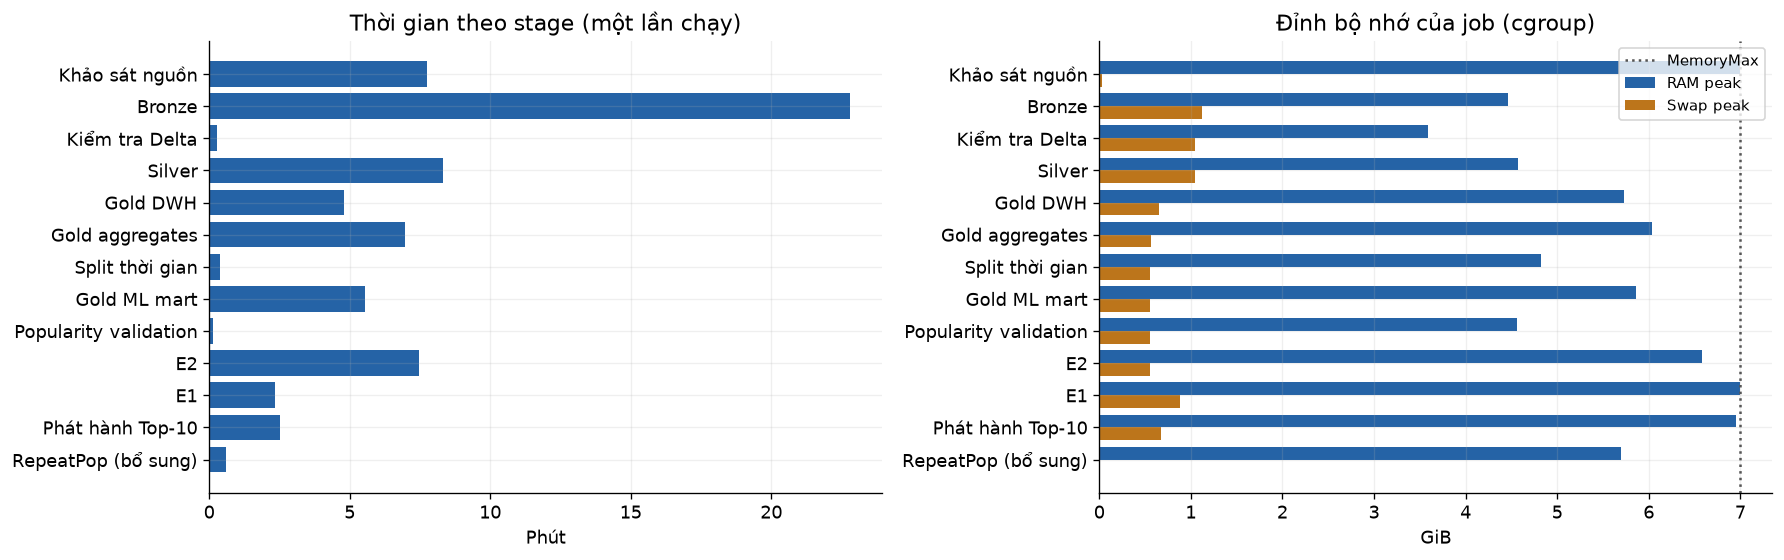
\includegraphics[width=\linewidth]{figures/output_09.png}
\caption{Thời gian và bộ nhớ đỉnh theo từng giai đoạn của lượt chạy toàn bộ dữ liệu}\label{fig:perf}
\end{figure}

% ════════════════════════════ KẾT LUẬN ═════════════════════════════════
\unnumbered{Kết luận và hướng phát triển}

\subsection*{1. Kết quả đạt được}
Về hạ tầng dữ liệu, đề tài đã xây dựng hoàn chỉnh pipeline Medallion trên Delta Lake và MinIO, xử lý toàn bộ 267 triệu sự kiện trên một máy giới hạn 7 GiB RAM trong khoảng 70 phút. Các kiểm tra xác nhận dữ liệu không mất, không trùng, tái lập được theo phiên bản; kho Star Schema bảo toàn đúng số sự kiện và phục vụ phân tích bằng Spark SQL.

Về mô hình, Implicit ALS trên GPU huấn luyện chỉ trong vài giây nhưng không vượt được Popularity về độ chính xác trên dữ liệu và lưới tham số đã khảo sát, dù cá nhân hóa hơn nhiều. Kết quả này khẳng định lại nhận định rằng mô hình đơn giản là mốc khó vượt trong bài toán Top-N, đặc biệt với hàng tiêu dùng có nhu cầu tập trung. Phân tích khám phá với RepeatPop gợi ý rằng lịch sử mua của chính user là tín hiệu mạnh nhất trong các phương pháp đã thử.

\subsection*{2. Hạn chế}
\begin{itemize}
  \item Chỉ có một mốc test và một lần đo thời gian; kết quả chưa được kiểm tra trên các cửa sổ thời gian khác.
  \item Lưới tham số hữu hạn và cấu hình tốt nhất nằm ở góc lưới.
  \item RepeatPop là phân tích khám phá, được thiết kế sau khi xem kết quả test.
  \item Dữ liệu đã ẩn danh, thời gian tương đối; hệ thống chạy trên một máy nên chưa suy rộng được cho cụm nhiều máy.
\end{itemize}

\subsection*{3. Hướng phát triển}
\begin{itemize}
  \item Thử độ tin cậy dạng logarit và mở rộng lưới tham số (rank nhỏ hơn, $\alpha$ nhỏ hơn, $\lambda$ lớn hơn).
  \item Kết hợp lịch sử mua với ALS: giữ sản phẩm mua lặp và dùng ALS cho các vị trí còn lại.
  \item Đánh giá trên nhiều mốc thời gian, đo tỷ lệ mua lặp thật của nhãn, và dùng thuộc tính sản phẩm cho user mới.
  \item Triển khai pipeline trên cụm nhiều máy.
\end{itemize}

% ════════════════════════ TÀI LIỆU THAM KHẢO ═══════════════════════════
\clearpage
\phantomsection\addcontentsline{toc}{chapter}{Tài liệu tham khảo}
\renewcommand{\bibname}{Tài liệu tham khảo}
\begin{thebibliography}{99}\setlength{\itemsep}{0pt}\markboth{Tài liệu tham khảo}{}
\bibitem{tecd} T-Tech, \emph{T-ECD Dataset}, Small Retail, revision \texttt{79bcf78}. \url{https://huggingface.co/datasets/t-tech/T-ECD}.
\bibitem{hu} Y. Hu, Y. Koren, C. Volinsky, “Collaborative Filtering for Implicit Feedback Datasets,” \emph{ICDM}, 2008, pp. 263–272.
\bibitem{rankingmetrics} Apache Spark, \emph{RankingMetrics}, tài liệu PySpark 4.2.0.
\bibitem{deltacompat} Delta Lake, \emph{Compatibility with Apache Spark}. \url{https://docs.delta.io/releases/}.
\bibitem{deltadocs} Delta Lake, \emph{Documentation}. \url{https://docs.delta.io/}.
\bibitem{medallion} Databricks, \emph{Medallion Architecture}. \url{https://docs.databricks.com/aws/en/lakehouse/medallion}.
\bibitem{s3a} Apache Hadoop, \emph{Hadoop-AWS: S3A}, phiên bản 3.5.0.
\bibitem{sparksql} Apache Spark, \emph{Spark SQL Programming Guide}, phiên bản 4.2.0.
\bibitem{spark} M. Zaharia et al., “Apache Spark: A Unified Engine for Big Data Processing,” \emph{Communications of the ACM}, 59(11), 2016, pp. 56–65.
\bibitem{delta} M. Armbrust et al., “Delta Lake: High-Performance ACID Table Storage over Cloud Object Stores,” \emph{PVLDB}, 13(12), 2020, pp. 3411–3424.
\bibitem{kimball} R. Kimball, M. Ross, \emph{The Data Warehouse Toolkit}, 3rd ed., Wiley, 2013.
\bibitem{koren} Y. Koren, R. Bell, C. Volinsky, “Matrix Factorization Techniques for Recommender Systems,” \emph{IEEE Computer}, 42(8), 2009, pp. 30–37.
\bibitem{takacs} G. Takács, I. Pilászy, D. Tikk, “Applications of the Conjugate Gradient Method for Implicit Feedback Collaborative Filtering,” \emph{RecSys}, 2011, pp. 297–300.
\bibitem{cremonesi} P. Cremonesi, Y. Koren, R. Turrin, “Performance of Recommender Algorithms on Top-N Recommendation Tasks,” \emph{RecSys}, 2010, pp. 39–46.
\bibitem{dacrema} M. Ferrari Dacrema, P. Cremonesi, D. Jannach, “Are We Really Making Much Progress? A Worrying Analysis of Recent Neural Recommendation Approaches,” \emph{RecSys}, 2019, pp. 101–109.
\bibitem{krichene} W. Krichene, S. Rendle, “On Sampled Metrics for Item Recommendation,” \emph{KDD}, 2020, pp. 1748–1757.
\bibitem{repeat} A. Anderson, R. Kumar, A. Tomkins, S. Vassilvitskii, “The Dynamics of Repeat Consumption,” \emph{WWW}, 2014, pp. 419–430.
\bibitem{ndcg} K. Järvelin, J. Kekäläinen, “Cumulated Gain-Based Evaluation of IR Techniques,” \emph{ACM TOIS}, 20(4), 2002, pp. 422–446.
\end{thebibliography}

\end{document}
